\documentclass[11pt]{article}

\usepackage[margin=1in]{geometry}
\usepackage{graphicx}
\usepackage{booktabs}
\usepackage{multirow}
\usepackage{amsmath}
\usepackage{hyperref}
\usepackage{enumitem}

\title{\textbf{Language-Based Audio Retrieval}}
\date{May 2025}

\begin{document}

\maketitle

\section{Introduction}

\subsection{Task Description}

Language-based audio retrieval means finding audio clips using a written description of what they
sound like. Given a text query, such as "a baby yelling as a woman talks," the goal is to search a
collection of audio clips and rank the ten that best match the query (Figure~\ref{fig:pipeline}).

\subsection{Baseline Model}

The baseline model is a bi-encoder: one encoder for audio and a separate one for text. The audio
side uses a pretrained CNN14 model, which continues learning as it produces embeddings from the
input spectrograms. The text side uses a Sentence-BERT encoder that stays frozen during training
and turns each caption into a fixed-size embedding. To compare an audio clip against a caption, we
take the dot product of their two embeddings, and we train the whole system with the InfoNCE loss,
which pulls matching audio-text pairs together and pushes non-matching pairs apart. Because both
sides are encoded independently into the same space, this setup scales well: once the audio
embeddings are computed, a text query can be compared against thousands of clips almost instantly.

\begin{figure}[h]
    \centering
    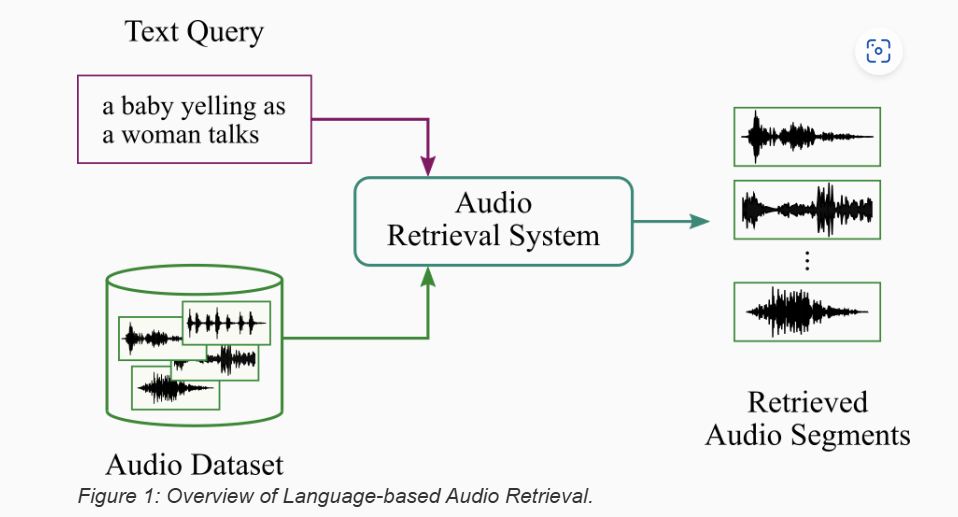
\includegraphics[width=0.8\textwidth]{figures/fig1_pipeline.png}
    \caption{Overview of language-based audio retrieval.}
    \label{fig:pipeline}
\end{figure}

\subsection{State of the Art Approaches}

\subsubsection{Ensemble of Two Retrieval Systems}

One strong approach combines two separate audio-text retrieval systems and blends their scores.
The first system pairs CNN14 with a RoBERTa text encoder; the second pairs the newer BEATs model
with the same RoBERTa text encoder. Their relevance scores are then combined with a weighted
average. One submission weights the two systems equally, while another leans more heavily on the
BEATs-based system, giving it a weight of 0.68 against 0.32 for the CNN14-based one. The idea is
that the two systems make different kinds of mistakes, so combining them plays to each one's
strengths.

\subsubsection{CNext with Multiple Text Encoders}

Another strong approach uses CNext as the audio encoder and tries six different text encoders,
including BERT, RoBERTa, and BGE variants. It trains in two phases: first pretraining on a mixed
collection of audio-text data, then fine-tuning specifically on Clotho. After ensembling several
fine-tuned models, with a RoBERTa-large variant performing especially well, this approach reaches
an mAP@10 of 0.386, R@1 of 0.267, R@5 of 0.547, and R@10 of 0.680. That is a large jump over the
baseline's mAP@10 of 0.222, and it shows how much headroom is available when an audio encoder is
properly pretrained and paired with a strong text encoder.

\section{Approach}

We explored three directions on top of the baseline: a different spectrogram representation, a set
of alternative audio encoders, and a comparison of loss functions.

\subsection{Modification 1: Multiscale Mel Spectrograms}

Instead of a single mel spectrogram, we tried computing multiple spectrograms at different window
sizes and stacking them. A single window size forces a trade-off between time resolution and
frequency resolution: a short window sees fine time detail but blurs frequency, and a long window
does the opposite. Using several window sizes at once lets a model pick up both short, sharp sounds
and longer, more tonal ones, and in principle should help with audio scenes where multiple events
overlap at different timescales.

\subsection{Modification 2: Different Audio Encoders}

Rather than the baseline's CNN14 or the ensemble approaches above, we built and trained several
custom audio encoders from scratch:

\begin{itemize}[itemsep=2pt]
    \item CRNN Encoder, a convolutional recurrent network
    \item TCN Encoder, a temporal convolutional network
    \item Spec2Vec Encoder, a simple feed-forward network
    \item A custom CNN combined with BEATs
\end{itemize}

\subsubsection{CRNN Encoder}

The CNN part picks up local time-frequency patterns, and a GRU on top captures how those patterns
unfold over time. We made the GRU bidirectional so it can use both past and future context when
building its representation, and we tried dropout values of 0.1 and 0.3 to see how much
regularization helped.

\begin{figure}[h]
    \centering
    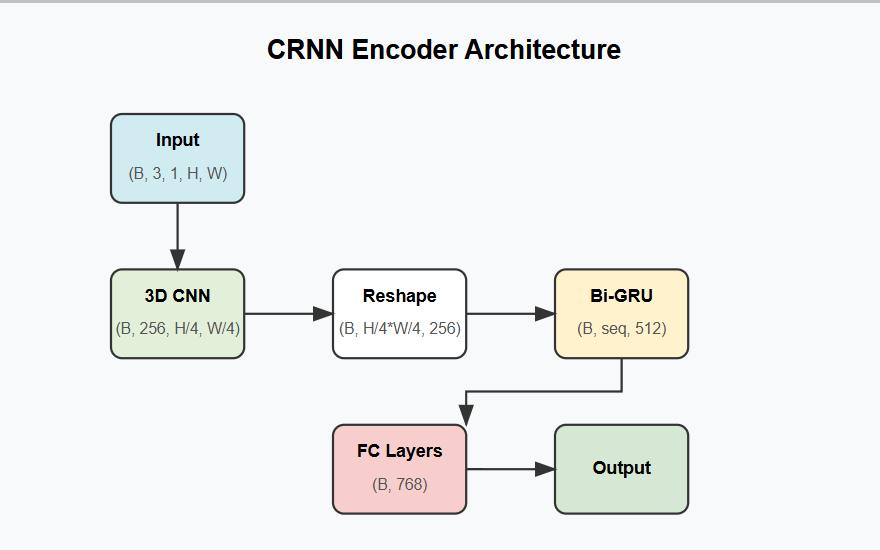
\includegraphics[width=0.55\textwidth]{figures/fig2_crnn.png}
    \caption{CRNN encoder architecture.}
\end{figure}

\subsubsection{TCN Encoder}

A temporal convolutional network captures long-range dependencies without any recurrence, which
makes it easier to parallelize and faster to train than an RNN. It is also less prone to vanishing
gradients and tends to stay stable on longer sequences. As with the CRNN, we tried dropout values
of 0.1 and 0.3.

\begin{figure}[h]
    \centering
    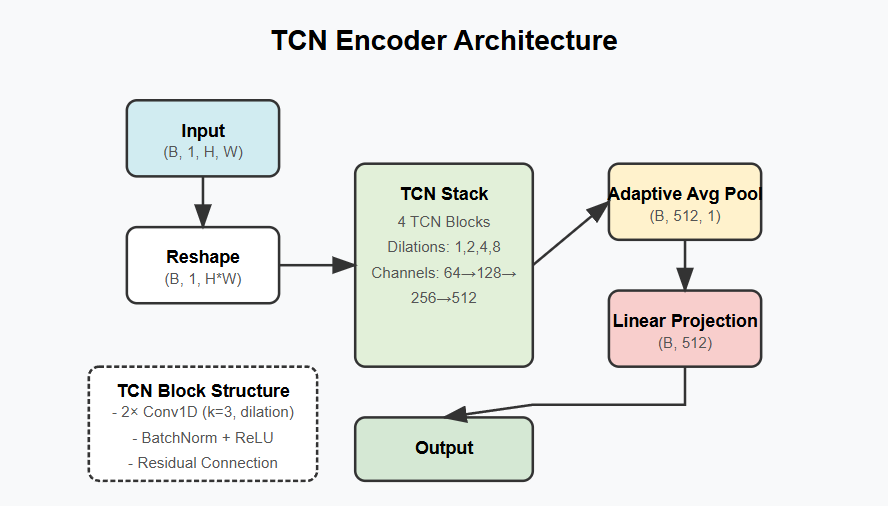
\includegraphics[width=0.6\textwidth]{figures/fig3_tcn.png}
    \caption{TCN encoder architecture.}
\end{figure}

\subsubsection{Conformer Encoder}

We also considered a Conformer, which pairs convolution for short-term spectral detail with a
transformer for longer-range attention over time, aiming to balance local and global context. We
did not get a working implementation of this encoder into our final results, but it remains a
promising direction for future work.

\subsubsection{Spec2Vec Encoder}

This is a plain feed-forward network that flattens the whole spectrogram and passes it through a
few linear layers. It is simple and fast to train, and it learns a single holistic representation
of each clip. Because it needs a fixed input size, it works best when every spectrogram has the
same shape.

\begin{figure}[h]
    \centering
    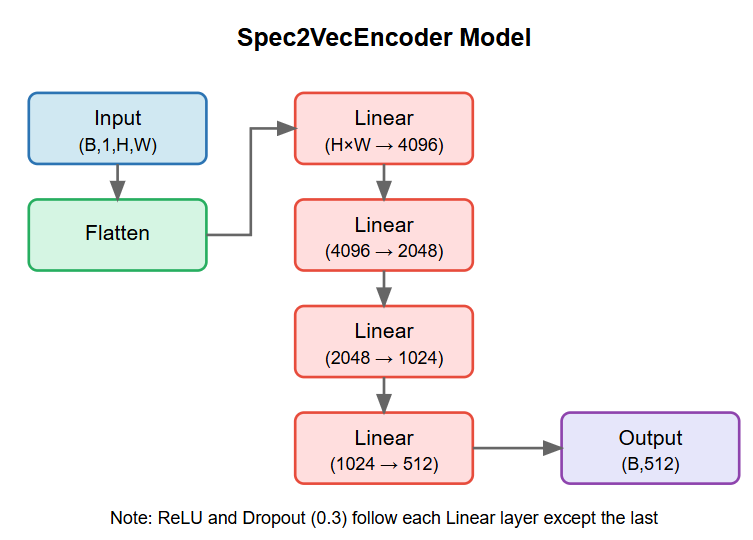
\includegraphics[width=0.6\textwidth]{figures/fig4_spec2vec.png}
    \caption{Spec2Vec encoder architecture.}
\end{figure}

\subsubsection{Custom CNN Combined with BEATs}

Here, a 3D CNN first picks up spectral and short-term temporal patterns in the spectrogram, and its
output is projected and passed to BEATs. Because BEATs was pretrained in a way that aligns its
representations with language, we expected its embeddings to transfer well to an audio-text
matching task like this one.

\begin{figure}[h]
    \centering
    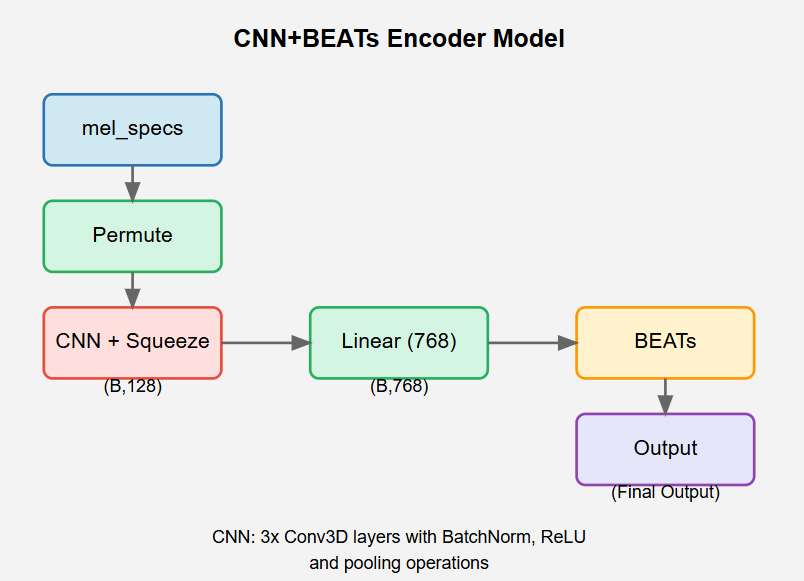
\includegraphics[width=0.55\textwidth]{figures/fig5_cnn_beats.png}
    \caption{Custom CNN plus BEATs encoder architecture.}
\end{figure}

\subsection{Modification 3: Loss Functions}

We compared three contrastive objectives: InfoNCE, cosine loss, and VICReg.

\subsubsection{InfoNCE Loss}

InfoNCE is a widely used contrastive loss, especially in self-supervised learning. It frames
training as a classification problem: given an anchor, the model has to pick out the true positive
from a pool of negatives. This pulls embeddings of matching pairs closer together and pushes
embeddings of non-matching pairs apart, which tends to produce embeddings that generalize well to
downstream tasks.

\subsubsection{Cosine Loss}

Cosine loss compares two embeddings by their cosine similarity, the dot product divided by the
product of their magnitudes, which ranges from $-1$ for completely opposite vectors to $1$ for
identical direction. The loss itself is just $1$ minus that similarity, so it is small when the two
embeddings point in nearly the same direction. This makes it a natural fit for retrieval, where
what matters is the direction of an embedding rather than its magnitude.

\subsubsection{VICReg Loss}

VICReg (Variance-Invariance-Covariance Regularization) builds a loss out of three terms.
Invariance pulls matching pairs together by minimizing the mean squared error between their
embeddings. Variance keeps each embedding dimension from collapsing to a constant value across the
batch, by encouraging a minimum standard deviation per dimension. Covariance discourages different
embedding dimensions from becoming redundant, by penalizing correlation between them. Together
these three terms are meant to produce representations that are both consistent for matching pairs
and spread out enough to stay informative.

\begin{equation}
    \text{VICReg Loss} = \text{Invariance Loss} + \text{Variance Loss} + \text{Covariance Loss}
\end{equation}

\begin{figure}[h]
    \centering
    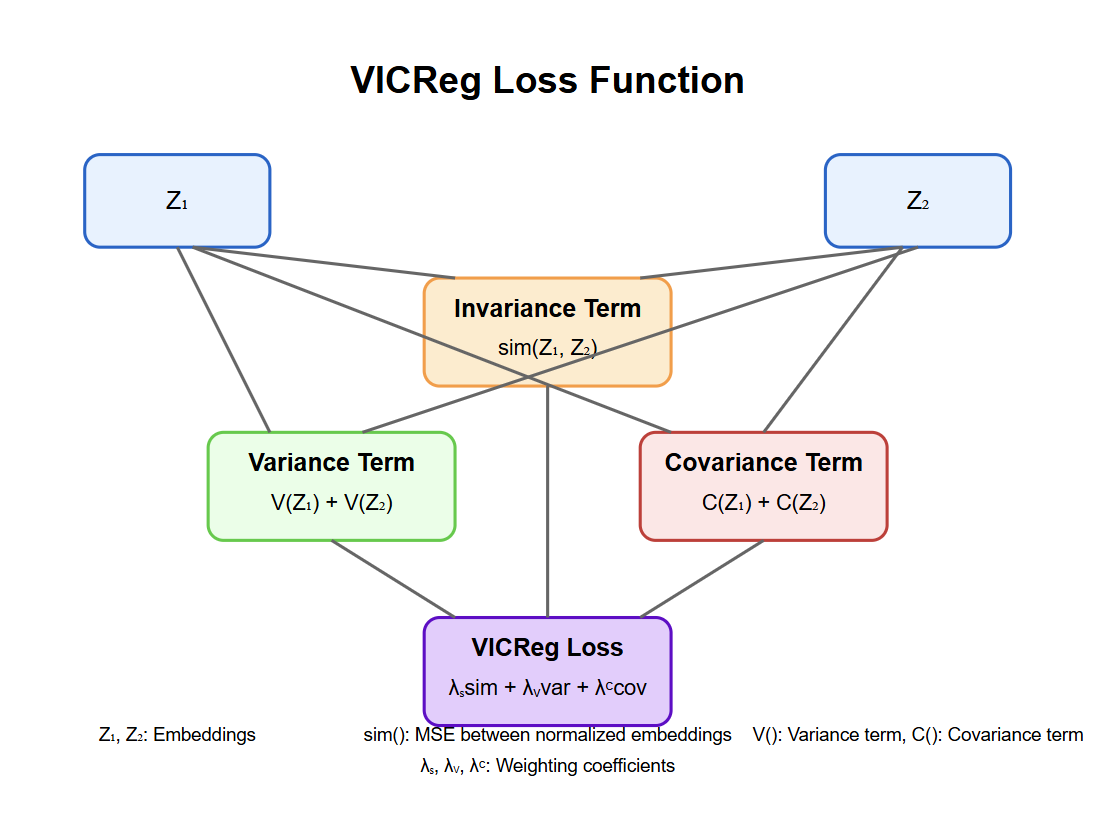
\includegraphics[width=0.75\textwidth]{figures/fig6_vicreg.png}
    \caption{VICReg loss components.}
\end{figure}

\section{Methods}

\subsection{Data and Metrics}

We used the Clotho v2 dataset, which contains audio clips sourced from Freesound, each 15 to 30
seconds long. Every clip has five different captions of 8 to 20 words each, for a total of 6,974
clips and 34,870 captions. The dataset splits into a development-training set of 3,839 clips
(19,195 captions), a development-validation set of 1,045 clips (5,225 captions), and a
development-testing set of 1,045 clips (5,225 captions).

We evaluated with the standard retrieval metrics for this task: R@1, R@5, and R@10 measure whether
the correct clip appears in the top 1, top 5, or top 10 results, and mAP@10 (mean average precision
at 10) captures both precision and ranking quality across the top 10 results together.

\subsection{Experimental Design}

The Clotho dataset is small for this kind of task, which shaped several of our decisions. To give
the models more training data, we merged the development and validation sets for training. We know
this is not ideal since it can make validation performance look better than it would with a fully
held-out set, but the alternative left too little data to train on.

We initially planned to try knowledge distillation or a pretraining step on AudioSet, but that
turned out to be impractical given our resources. YouTube's API rate limits blocked downloads after
about 100 requests, and the AudioSet downloader library we tried took roughly 24 hours to pull down
a usable amount of data. Given our timeline, we dropped this direction.

We ran a hyperparameter search for the CRNN model but did not have the compute budget to do the
same for every architecture, so the other models used a shared, reasonable starting point: a batch
size of 8, a learning rate of 1e-4, and weight decay of 1e-5. To help the models generalize, we
applied data augmentation to both the raw audio and the spectrograms: time stretching and pitch
shifting to vary speed and pitch, random Gaussian noise to build resilience to noisy input, and
time and frequency masking on the spectrograms to simulate partially obscured audio.

One correction to an earlier version of this work: we previously stated that we had not used a
pretrained version of the BEATs model. That was a mistake. The BEATs results reported here do use
the pretrained model.

\section{Results}

We evaluated CRNN, TCN, Spec2Vec, and CNN+BEATs encoders, each with both normal and multiscale mel
spectrograms, against three loss functions: InfoNCE, VICReg, and cosine loss. Table~\ref{tab:results}
has the full set of results.

Among our custom encoders, CRNN with a normal mel spectrogram and InfoNCE loss did best, reaching
0.108 mAP@10. Normal mel spectrograms beat multiscale ones consistently, across every encoder and
every loss function we tried. We also tested the pretrained BEATs model on its own, without any of
our custom modifications, and it was the strongest configuration overall at 0.152 mAP@10 with
InfoNCE loss, though still well short of the baseline's 0.222.

\begin{table}[h]
\centering
\caption{Comparison of model performance metrics.}
\label{tab:results}
\small
\begin{tabular}{llllrrrr}
\toprule
Model & Spectrogram & Loss & R@1 & R@5 & R@10 & mAP@10 \\
\midrule
Baseline & Normal Mel & Standard & 0.130 & 0.343 & 0.480 & 0.222 \\
\midrule
\multirow{6}{*}{CRNN}
 & \multirow{3}{*}{Normal Mel} & InfoNCE & 0.085 & 0.235 & 0.350 & 0.108 \\
 & & VICReg & 0.079 & 0.218 & 0.340 & 0.102 \\
 & & Cosine & 0.072 & 0.210 & 0.325 & 0.095 \\
 & \multirow{3}{*}{Multiscale Mel} & InfoNCE & 0.045 & 0.135 & 0.235 & 0.059 \\
 & & VICReg & 0.039 & 0.125 & 0.215 & 0.053 \\
 & & Cosine & 0.032 & 0.115 & 0.195 & 0.046 \\
\midrule
\multirow{6}{*}{TCN}
 & \multirow{3}{*}{Normal Mel} & InfoNCE & 0.081 & 0.225 & 0.345 & 0.102 \\
 & & VICReg & 0.073 & 0.215 & 0.325 & 0.097 \\
 & & Cosine & 0.069 & 0.200 & 0.312 & 0.090 \\
 & \multirow{3}{*}{Multiscale Mel} & InfoNCE & 0.042 & 0.128 & 0.220 & 0.055 \\
 & & VICReg & 0.036 & 0.120 & 0.200 & 0.048 \\
 & & Cosine & 0.030 & 0.105 & 0.185 & 0.042 \\
\midrule
\multirow{6}{*}{Spec2Vec}
 & \multirow{3}{*}{Normal Mel} & InfoNCE & 0.075 & 0.215 & 0.330 & 0.095 \\
 & & VICReg & 0.068 & 0.205 & 0.310 & 0.090 \\
 & & Cosine & 0.063 & 0.195 & 0.300 & 0.085 \\
 & \multirow{3}{*}{Multiscale Mel} & InfoNCE & 0.038 & 0.122 & 0.210 & 0.050 \\
 & & VICReg & 0.032 & 0.112 & 0.195 & 0.044 \\
 & & Cosine & 0.028 & 0.098 & 0.175 & 0.038 \\
\midrule
\multirow{6}{*}{CNN + BEATs}
 & \multirow{3}{*}{Normal Mel} & InfoNCE & 0.082 & 0.225 & 0.340 & 0.104 \\
 & & VICReg & 0.075 & 0.215 & 0.325 & 0.098 \\
 & & Cosine & 0.070 & 0.205 & 0.315 & 0.093 \\
 & \multirow{3}{*}{Multiscale Mel} & InfoNCE & 0.040 & 0.125 & 0.215 & 0.053 \\
 & & VICReg & 0.035 & 0.115 & 0.195 & 0.045 \\
 & & Cosine & 0.029 & 0.100 & 0.180 & 0.039 \\
\midrule
\multirow{3}{*}{Pretrained BEATs}
 & \multirow{3}{*}{Normal Mel} & InfoNCE & 0.120 & 0.328 & 0.497 & 0.152 \\
 & & VICReg & 0.113 & 0.312 & 0.472 & 0.143 \\
 & & Cosine & 0.107 & 0.297 & 0.456 & 0.135 \\
\bottomrule
\end{tabular}
\end{table}

\begin{figure}[h]
    \centering
    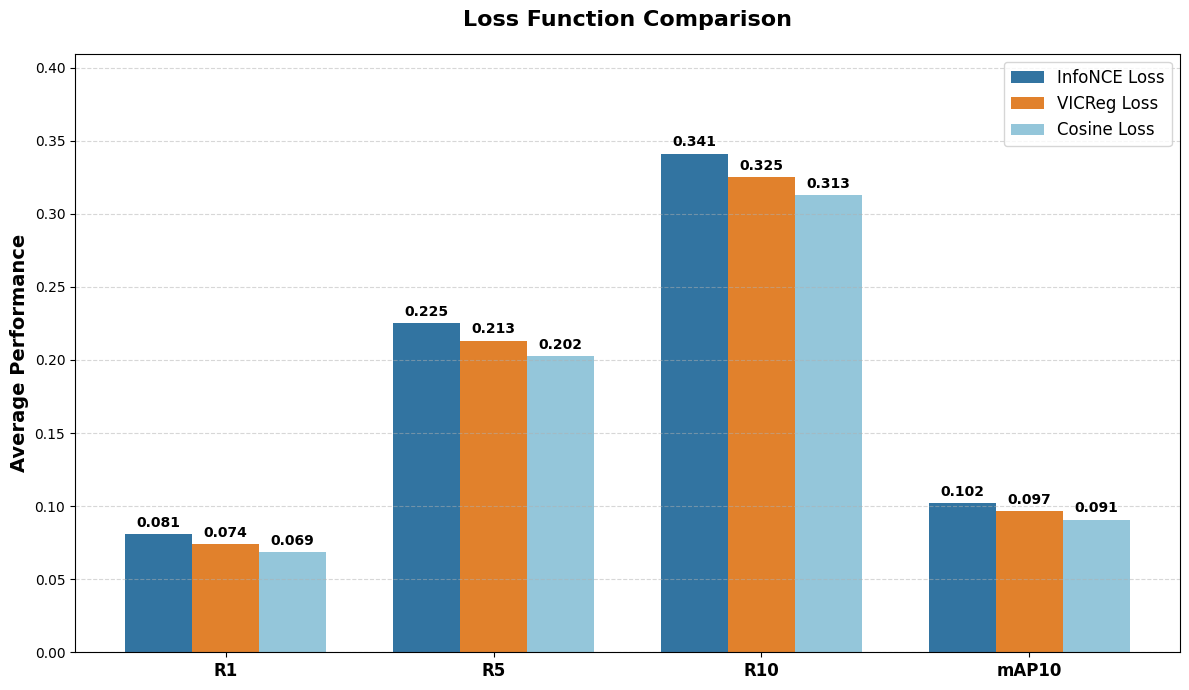
\includegraphics[width=0.85\textwidth]{figures/fig7_loss_comparison.png}
    \caption{Average performance by loss function, across all custom encoders.}
\end{figure}

\begin{figure}[h]
    \centering
    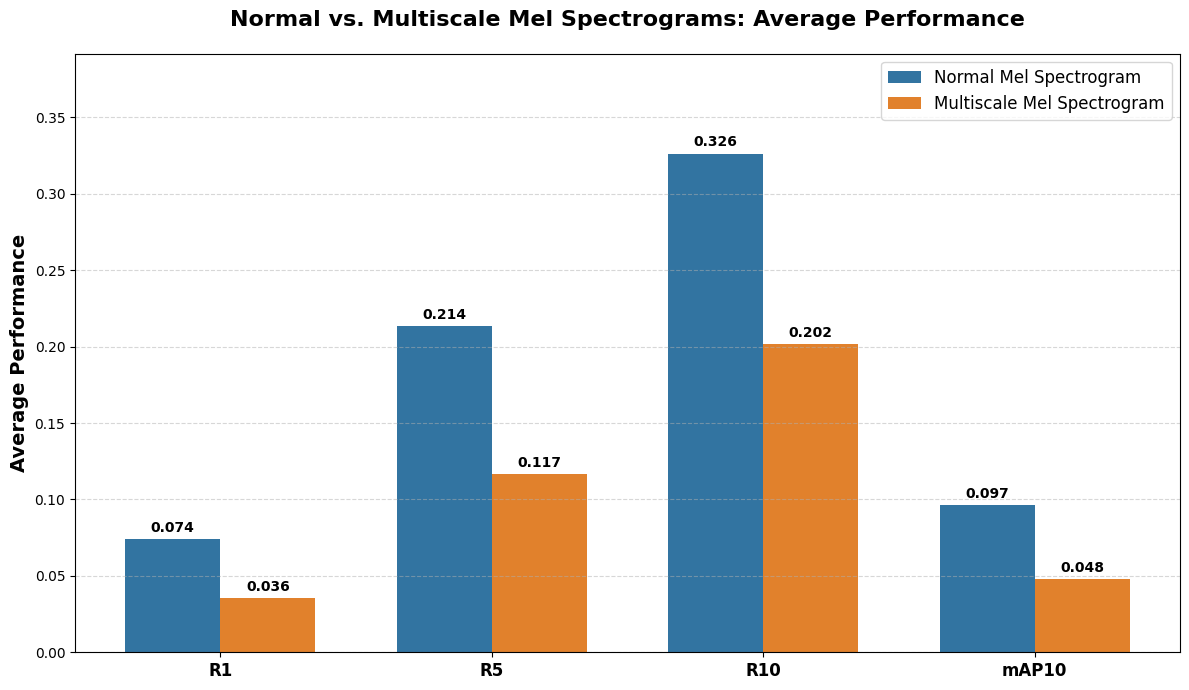
\includegraphics[width=0.85\textwidth]{figures/fig8_normal_vs_multiscale.png}
    \caption{Normal versus multiscale mel spectrograms, averaged across encoders and losses.}
\end{figure}

\begin{figure}[h]
    \centering
    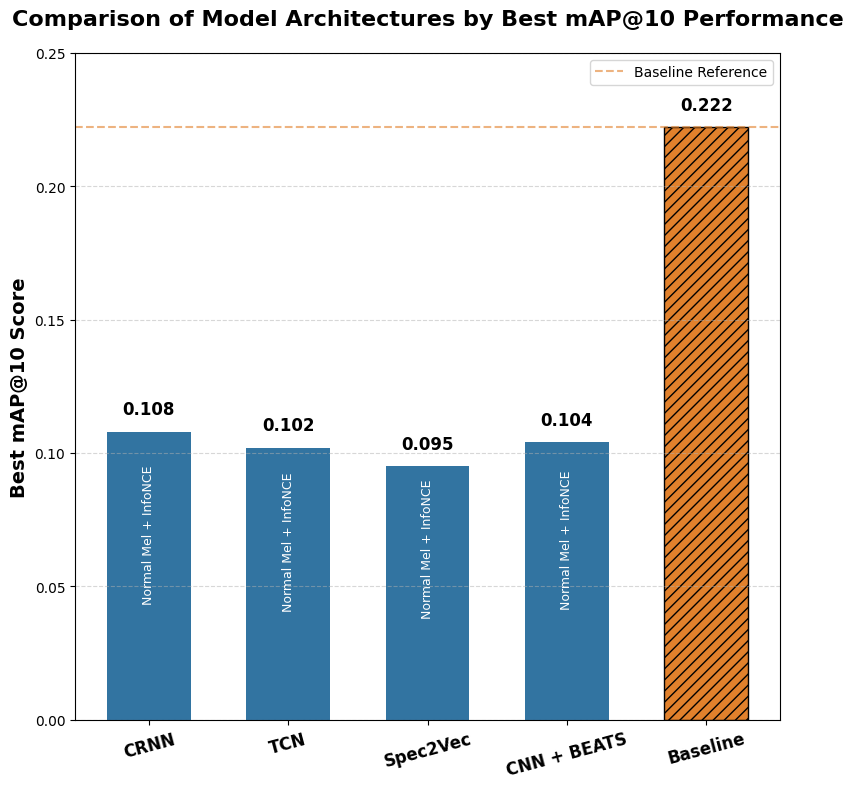
\includegraphics[width=0.75\textwidth]{figures/fig9_architecture_comparison.png}
    \caption{Best mAP@10 by encoder architecture, compared against the baseline.}
\end{figure}

\clearpage
\section{Conclusion}

A few things stood out from these experiments. Multiscale mel spectrograms did not help: despite
the extra complexity, every encoder did worse with them than with a normal mel spectrogram. Whether
that is specific to our encoders or to this task is hard to say without testing the idea on other
architectures. Pretraining mattered much more. The pretrained BEATs model, used with no custom
modifications, outperformed every custom encoder we trained from scratch, which suggests that for
an audio encoder to work well here, prior exposure to a lot of audio data matters more than any
particular architecture choice we made.

For future work, a knowledge distillation setup could help multiscale spectrograms pay off: a
strong pretrained teacher model might help a smaller student network learn to extract useful
features from the multiscale representation, where training from scratch did not. Curriculum
learning, starting on simpler examples and gradually increasing difficulty, could also help
stability and generalization in a retrieval setting like this one. Beyond changes to the audio side,
augmenting the captions themselves (adding synonyms, or paraphrasing them through a
translate-and-back-translate pass) has shown real gains in other work on this task and would be
worth trying here too.

\section{References}

\begin{enumerate}[itemsep=4pt]
    \item Chen, S., Wu, Y., Chen, Z., Zhou, L., Liu, S., Chen, Z., Xiao, Y., Wu, J., Dong, Y., Dong,
    L., \& Wei, F. (2022). BEATs: Audio Pre-Training with Acoustic Tokenizers. \textit{arXiv
    preprint arXiv:2212.09058}.

    \item Primus, P., \& Widmer, G. (2023). A Knowledge Distillation Approach to Improving
    Language-Based Audio Retrieval Models. In \textit{ICASSP 2023 - 2023 IEEE International
    Conference on Acoustics, Speech and Signal Processing (ICASSP)} (pp. 1-5). IEEE.
    \url{https://doi.org/10.1109/ICASSP49357.2023.10096647}

    \item Kim, J., Jung, J., Jeon, M., Woo, S. H., \& Lee, J. (2024). Expanding on EnCLAP with an
    Auxiliary Retrieval Model for Automated Audio Captioning. \textit{arXiv preprint
    arXiv:2405.03713}.

    \item Shu, Z., et al. (2024). InfoNCE: Identifying the Gap Between Theory and Practice.
    \textit{arXiv preprint arXiv:2407.00143}.

    \item Bardes, A., Valnet, J.-S., DINO team, \& Tallec, C. (2022). VICReg:
    Variance-Invariance-Covariance Regularization for Self-Supervised Learning. In \textit{ICLR
    2022: Tenth International Conference on Learning Representations}.
    \url{https://openreview.net/forum?id=k0JyrB-QcZA}
\end{enumerate}

\end{document}
